\documentclass[tikz,border=6mm]{standalone}

\begin{document}

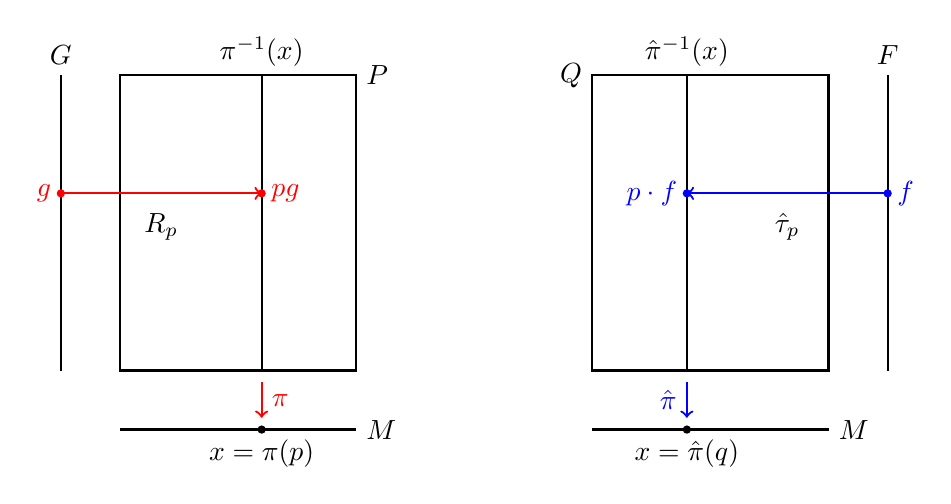
\begin{tikzpicture}[scale=1.5]

% Outer rectangle for the fiber bundle
  \draw[thick] (-4,0) rectangle (-2,2.5) node[right] {$P$};
% Base manifold (M)
\draw[thick] (-4,-0.5) -- (-2,-0.5) node[right] {$M$};
\draw[thick] (-4.5,0) -- (-4.5,2.5) node[above] {$G$};
% Highlight one tangent space TxM
\draw[thick] (-2.8,0) -- (-2.8,2.5);
\node at (-2.8,2.7) {$\pi^{-1}(x)$};
\fill[red] (-2.8,1.5) circle (1pt) node[right] {$pg$};
\fill[red] (-4.5,1.5) circle (1pt) node[left]{$g$};

\draw[red,->,thick](-4.5,1.5) -- (-2.8, 1.5) node[black,pos = 0.5,below,yshift = -3.5]{$R_p$};
% Labels
\fill (-2.8,-0.5) circle (1pt);
\node[below] at (-2.8,-0.5) {$x = \pi(p)$};
% Projection arrow (pi)
\draw[red,->,thick] (-2.8,-0.1) -- (-2.8,-0.4) node[midway,right] {$\pi$};

% Outer rectangle for the fiber bundle
\draw[thick] (2,0) rectangle (0,2.5) node[left] {$Q$};
% Base manifold (M)
\draw[thick] (0,-0.5) -- (2,-0.5) node[right] {$M$};
\draw[thick] (2.5,0) -- (2.5,2.5) node[above] {$F$};
% Highlight one tangent space TxM
\draw[thick] (0.8,0) -- (0.8,2.5);
\node at (0.8,2.7) {$\hat{\pi}^{-1}(x)$};
\fill[blue] (0.8,1.5) circle (1pt) node[left] {$p\cdot f$};
\fill[blue] (2.5,1.5) circle (1pt) node[right]{$f$};

\draw[blue,->,thick](2.5,1.5) -- (0.8, 1.5) node[black,pos = 0.5,below,yshift = -3.5]{$\hat{\tau}_p$};
% Labels
\fill (0.8,-0.5) circle (1pt);
\node[below] at (0.8,-0.5) {$x = \hat{\pi}(q)$};
% Projection arrow (pi)
\draw[blue,->,thick] (0.8,-0.1) -- (0.8,-0.4) node[midway,left] {$\hat{\pi}$};

\end{tikzpicture}

\end{document}
